\documentclass[12pt, a4paper]{article}

\usepackage[english]{babel}
\usepackage{amsmath}
\usepackage{amssymb}
\usepackage{amsthm}
\usepackage{graphicx}
\usepackage{hyperref}
\usepackage{geometry}
\geometry{
	a4paper,
	left=20mm,
	right=20mm,
	top=25mm,
	bottom=25mm
}


\title{pestim - an R package to estimate population counts from aggregated mobile phone data}
\author{David Salgado\footnote{Department of Methodology and Development of Statistical Production, Statistics Spain (INE)}  and who else to add as author??}

\date{}


\begin{document}
\maketitle

\begin{abstract}
This package has been developed in the context of a European research project 
within the European Statistical System called ESSnet on Big Data.
It provides an implementation for a hierarchical model to combine both 
aggregated mobile phone data and external official (administrative or survey) 
data to produce estimates of population counts in each cell of a division of a territory using a Bayesian approach.
\end{abstract}


\section{Introduction}

\texttt{pestim} R package implements a hierarchical model to estimate the population counts of different territorial cells 
combining the information from aggregated 
mobile phone data and a population register or survey data, both at a given time instant and along a 
sequence of time periods. The theoretical model implemented by the \texttt{pestim} R package
follows the ecological sampling techniques to estimate population counts (see e.g. \cite{ManNacAlb15a} and 
\cite{RoyDor08a}) which are based on a bayesian approach. The complete methodology is described in \cite{methodology}.
The proposed model rests on two working assumptions:
\begin{itemize}
	\item Given that mobile phone data and official data operate at different 
time scales, we assume that there exists an initial time instant 
in which we can equate population figures from both sources.
	\item The mobility patterns of individuals do not depend on the mobile 
network operator which they are subscribed to.
\end{itemize}

The inference of the population counts from mobile phone data and official data is achieved in a two step process:
\begin{itemize}
	\item {at a given time instant $t_{0}$ both mobile phone and 
official data are used to infer the population counts in each territorial cell;}
	\item {at later moments, $t_{1}, t_{2},...$ the transition probabilities are inferred from mobile phone 
	data and are used to estimate the spatial and time evolution of the population.}
\end{itemize}


The package is structured on three layers of functions:
\begin{itemize}
	\item \textbf{Auxiliary functions}, providing computation of mathematical functions 
such as the ratio of two beta functions, the confluent hypergeometric function, 
an optimization routine for a concrete probability distribution, etc. 
Examples of these functions are \texttt{ratioBeta, kummer, Phi, modeLambda};
	\item \textbf{Distribution-related functions}, providing computation regarding
the generation of random deviates according to different probability distributions 
comprising both priors, posteriors, and the generation of parameter specifications 
for these distributions. Examples of these functions are 
\texttt{dtriang, rtriang, ptriang, qtriang, dlambda, rlambda, rmatProb, rN0, rNt, rNtcondN0, rg, rp, alphaPrior, genAlpha, genUV}.
\item \textbf{Estimation-related functions}, providing computation of estimates 
based upon the populations generated with the preceding functions. 
Examples of these functions are \texttt{postN0, postNt, postNtcondN0}.
\end{itemize}

\texttt{pestim} package is freely available under the \texttt{GPL3} and \texttt{EUPL} lincese 
at the following address: \url{https://github.com/MobilePhoneESSnetBigData/pestim}. 
It can be installed using \texttt{install\_github()} function from \texttt{devtools} package:
\begin{verbatim}
library(devtools)
install_github("MobilePhoneESSnetBigData/pestim")
\end{verbatim}

Since it contains \texttt{C++} code, the user need to install \texttt{Rtools} under Windows 
enviroment or to have a  \texttt{C++}  compiler under Linux or Mac OS X environments.

\section{The hierarchical model}\label{model}

In this section we will give a short description of the theoretical model 
underlaying the \texttt{pestim} R package for estimation of the population 
counts at a given time moment.

A first input of the model is 
$\mathbf{N}^{\textrm{MNO}}=(N_{1}^{\textrm{MNO}}, \dots, N_{I}^{\textrm{MNO}})^{T}$ which 
represents the population counts reported by the mobile network operator in 
each territorial cell $i\in\mathcal{I}=\{1,\dots,I\}$ (i.e. the aggregated mobile phone data). 
The second input of the model is the official population counts in each territorial cell denoted by 
$\mathbf{N}^{\textrm{REG}}=(N_{1}^{\textrm{REG}}, \dots, N_{I}^{\textrm{REG}})^{T}$. 
These official population counts could come from administrative data sources or from statistical surveys.
\texttt{pestim} implements a function to estimate the actual population 
counts $\mathbf{N}=(N_{1}, \dots, N_{I})^{T}$ combining both data sources. 
It also computes the posterior probability distribution 
$\mathbb{P}\left(\mathbf{N}|\mathbf{N}^{\textrm{MNO}};\mathbf{N}^{\textrm{REG}}\right)$ 
that can be used to assess the uncertainty in the output estimates.
This process can be represented schematically as shown in figure \ref{Tool}.


\begin{figure}[htbp]
\centering
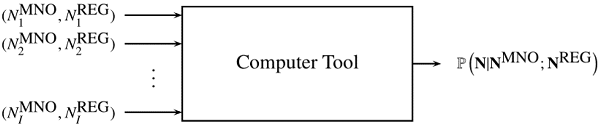
\includegraphics[scale=0.75]{Tool.png}
\caption{The diagram of the process for population estimation using mobile phone and official population data.}
\label{Tool} 
\end{figure}

The main idea of the model is to emulate the ecological sampling setting in which 
the number of detected individuals in each cell follows a binomial distribution $Bin(N_{i}, p_{i})$ 
whose parameter $N_{i}$ is the target of the model and is assigned a weakly informative prior 
and the detection probability $p_{i}$ is also assigned a weakly informative prior based 
upon both data sources. In our case, if we have $N_{i}$ individuals in cell $i$ and 
we have an independent detection probability $p_{i}$ for each individual through 
the mobile telecommunication network, then we will detect $N_{i}^{\textrm{MNO}}$ 
individuals according to the aggregated mobile phone data naturally following a binomial 
distribution. $N_{i}$  can be modeled as Poisson random variables with independent 
parameters $\lambda_{i}$, variables which are pairwise independent, while $p_{i}$ are 
the proportions of individuals detected by the MNO at time $t_{0}$ in each cell $i$. 
It is important to note here that $p_{i}$ is not simply the market share of the MNO in 
cell $i$ but the actual proportion of individuals detected by the network. As an 
example, a call between a subscriber in a cell $i$ and a non-subscriber in another 
cell $j$ of a given MNO is certainly detected by the network in \emph{\textbf{both cells}}, 
thus potentially being part of the aggregated data $N_{i}^{\textrm{MNO}}$ and $N_{j}^{\textrm{MNO}}$. 
This example emphasizes the importance  of the knowledge of the preprocessing and aggregation 
procedures from microdata for the final result.

The detection probabilities $p_{i}$ are modeled as $Beta$ distributed independently 
random variables with $\alpha_{i}$ and $\beta_{i}$ parameters in each cell. The prior 
distribution of the parameters $\alpha_{i}$ and $\beta_{i}$ comes from the following reasoning.
We assume that $\frac{\alpha_{i}}{\alpha_{i} + \beta_{i}}$ 
and $\alpha_{i} + \beta_{i}$ are independently distributed according 
to $\frac{\alpha_{i}}{\alpha_{i} + \beta_{i}}\simeq f_{1}(\frac{\alpha_{i}}{\alpha_{i}+\beta_{i}}; \mathbf{N}^{\textrm{REG}}, \mathbf{z})$   
and $\alpha_{i} + \beta_{i}\simeq f_{2}(\alpha_{i}+\beta_{i}; \mathbf{N}^{\textrm{REG}}, \mathbf{z})$.
Here  $f_{1}$ and $f_{2}$ are weakly informative prior distributions for $\frac{\alpha}{\alpha + \beta}$
and $\alpha + \beta$ and they made use of the information from the population 
register ($\mathbf{N}^{\textrm{REG}}$) and any other auxiliary information $\mathbf{z}$. 
The parameters $\alpha_{i}+\beta_{i}$ can be understood as the population size of 
each cell $N_{i}$ (thus with support in $(0,\infty)$) upon which the detection is executed 
at that time instant and $\alpha_{i}/(\alpha_{i}+\beta_{i})$ can be understood as a priori proportions 
of individuals detected by the MNO in cell $i$. 
If we assume $f_{2}$ to be a gamma distribution with parameters 
$(N_{i}^{\textrm{MNO}} + 1, \frac{N_{i}^{\textrm{MNO}}}{N_{i}^{\textrm{REG}}})$  the most probable 
value for the sample size is $N_{i}^{\textrm{REG}}$ which is consistent with the preceding hypothesis for $N_{i}$.
With no prior information about the detection probability we may assume $f_{1}=\textrm{Unif}[0,1]$.
the parameters $\lambda_{i}$ are modeled with another weakly information prior $f_{3}$ which may incorporate 
the information we have from the population register or similar sources.

Thus, the model can be summarized as follows:

\begin{align}\label{model1}
N_{i}^{\textrm{MNO}}&\simeq\textrm{Bin}\left(N_{i}, p_{i}\right),\qquad N_{i}^{\textrm{MNO}}\perp N_{j}^{\textrm{MNO}},\quad i\neq j=1,\dots,I\\
N_{i}&\simeq\textrm{Po}\left(\lambda_{i}\right),\qquad N_{i}\perp N_{j},\quad i\neq j=1,\dots,I\nonumber\\
p_{i}&\simeq\textrm{Beta}\left(\alpha_{i},\beta_{i}\right),\qquad p_{i}\perp p_{j}\quad i\neq j=1,\dots,I\nonumber\\
\left(\alpha_{i}, \beta_{i}\right)&\simeq \frac{f_{1}(\frac{\alpha_{i}}{\alpha_{i}+\beta_{i}}; \mathbf{N}^{\textrm{REG}}, \mathbf{z})\cdot f_{2}(\alpha_{i}+\beta_{i}; \mathbf{N}^{\textrm{REG}}, \mathbf{z})}{\alpha_{i}+\beta_{i}}\quad
(\alpha_{i},\beta_{i})\perp(\alpha_{j},\beta_{j}),\quad i\neq j=1,\dots,I\nonumber\\
\lambda_{i}&\simeq f_{3}(\lambda_{i}; N_{i}^{\textrm{REG}}, \mathbf{z})\quad (\lambda_{i} > 0, \lambda_{i}\perp\lambda_{j}), \quad i=1,\dots,I.\nonumber
\end{align}

The quantity of interest here is the target population counts $\mathbf{N}=(N_{1},\dots,N_{I})^{T}$ in each cell $i$. We will follow a Bayesian
approach to compute the posterior distribution of the target population. This approach allows us to  
account for the inference and the assessment of the uncertainty, hence of quality of estimations.
We can leverage the prior information we have at our disposal by choosing the probability distribution $f_{1}$, $f_{2}$ and $f_{3}$. 
The posterior distribution $\mathbb{P}\left(\mathbf{N}\big|\mathbf{N}^{\textrm{MNO}};\mathbf{N}^{\textbf{REG}}\right)$ is given by (we dropped the subscripts
since each cell is treated independently of each other) \cite{methodology}:

\begin{align}
\mathbb{P}\left(N\big|N^{\textrm{MNO}};N^{\textbf{REG}}\right)&\propto 
\label{PostProbN} \int_{0}^{\infty}d\lambda\quad\mathbb{P}\left(\lambda\big|N^{\textrm{MNO}};N^{\textbf{REG}}\right)\cdot\textrm{Po}(N; \lambda),
\end{align}

$N$ being a Poisson random variable, the most probable value for $N$ is given by $\lfloor \lambda\rfloor$ and the posterior 
distribution for the hyperparameter $\lambda$ will allow us to provide a point estimator for $N$ (mode, mean, median, \dots).

The posterior $\mathbb{P}\left(\lambda \big|\mathbf{N}^{\textrm{MNO}};\mathbf{N}^{\textbf{REG}}\right)$ is given by \cite{BDA3} \cite{methodology}:

\begingroup\small
\begin{align}\label{Sdef1}
\mathbb{P}\left(\lambda\big|N^{\textrm{MNO}};N^{\textbf{REG}}\right)&\propto \mathbb{P}\left(\lambda\right)\cdot \textrm{Po}(N^{\textrm{MNO}}; \lambda) \cdot S\left(\lambda, N^{\textrm{MNO}}, N^{REG}\right),
\end{align}
\endgroup

\noindent where we have defined 

\begingroup\small
\begin{align}\label{Sdef2}
S(\lambda, N^{\textrm{MNO}}, N^{\textrm{REG}}) &= \sum_{n = 0}^{\infty}\frac{\lambda^{n}}{n!}I_{N^{\textrm{MNO}}, n}(N^{\textrm{REG}}),\\
I_{N^{\textrm{MNO}}, n}(N^{\textrm{REG}})&=\int_{0}^{\infty}\int_{0}^{\infty}d\alpha d\beta\ \frac{f_{1}(\frac{\alpha}{\alpha+\beta}; N^{\textrm{REG}})\cdot f_{2}(\alpha+\beta; N^{\textrm{REG}}}{\alpha+\beta}\frac{B\left(\alpha+N^{\textrm{MNO}}, \beta+n- N^{\textrm{MNO}}\right)}{B\left(\alpha, \beta\right)}.
\end{align}
\endgroup

In order to compute the integral $I_{N^{\textrm{MNO}}, n}(N^{\textrm{REG}})$ we use 
a change of variables $u = \frac{\alpha}{\alpha + \beta}, v = \alpha + \beta$. The integral becomes \cite{methodology}:

\begin{align}
\label{MC}I_{n,m}(N^{\textrm{REG}})&= \int_{0}^{\infty}dv f_{2}(v)\int_{0}^{1}du\ f_{1}(u)\frac{B(u\cdot v + n, (1-u)\cdot v + m)}{B(u\cdot v, (1-u)\cdot v)}
\end{align}

This form of the integral allows us to use Monte Carlo technique. We consider the function 
$g_{n,m}(\mathbf{x})=\frac{B(x_{1}\cdot x_{2} + n, (1-x_{1})\cdot x_{2} + m)}{B(x_{1}\cdot x_{2}, (1-x_{1})\cdot x_{2})}$ 
and generate $M$ bidimensional random variables $\mathbf{x}\in[0,1]\times\mathbf{R}^{+}$ according to the bidimensional 
distribution $f_{1}\times f_{2}$. Then, using $f(\mathbf{x})=f_{1}(x_{1})f_{2}(x_{2})$ as importance function, 
we can write:
\begin{equation}
I_{n,m}(N^{\textrm{REG}})=\lim_{M\to\infty}\frac{1}{M}\sum_{i=1}^{M}g_{n,m}(\mathbf{x}_{i}).
\end{equation}

We made use of stratified importance sampling and introduced the stratification as follows: we defined $H_{1}\cdot H_{2}$ strata as the rectangular 
domains $[a_{h_{1}-1}, a_{h_{1}}]\times [b_{h_{2} -1}, b_{h_{2}}]$, where $a_{h_{1}}=F_{1}^{-1}\left(h_{1}/H_{1}\right)$ ($h_{1}=1, \dots, H_{1}$) and $b_{h_{2}}=F_{2}^{-1}\left(h_{2}/H\right)$ ($h_{2}=1, \dots, H_{2}$), 
and $F_{i}$ stands for the distribution function corresponding to the density function $f_{i}$. 
Defining the importance function in each stratum by $f_{h_{1}h_{2}}= H_{1}\cdot H_{2}\cdot f_{1}\cdot f_{2}$ 
truncated at $[a_{h_{1}-1}, a_{h_{1}}]\times[b_{h_{2}-1}, b_{h_{2}}]$ and taking equal-size strata $M_{h_{1}h_{2}}=\frac{M}{H_{1}H_{2}}$, 
then we obtained:

\begin{equation}
I_{n,m}(N^{\textrm{REG}})=\lim_{M\to\infty}\frac{1}{M}\sum_{h_{1}=1}^{H_{1}}\sum_{h_{2}=1}^{H_{2}}\sum_{i_{h_{1}}=1}^{M/H_{2}}\sum_{i_{h_{2}}=1}^{M/H_{1}}g_{n,m}(\mathbf{x}_{i_{h_{1}}i_{h_{2}}})
\end{equation}

\noindent where the random values $\mathbf{x}_{i_{h_{1}}i_{h_{2}}}$ are generated with the corresponding density function $f_{h_{1}h_{2}}$.

Once computed the integrals $I_{N^{\textrm{MNO}}, n}(N^{\textrm{REG}})$, the series $S(\beta_{0}, N^{\textrm{MNO}}, N^{\textrm{REG}})$ is summed up with standard procedures.

Another approach of computing $S(\beta_{0}, N^{\textrm{MNO}}, N^{\textrm{REG}})$ gives \cite{methodology}:

\begin{align}
S(\lambda, N^{\textrm{MNO}}, N^{\textrm{REG}})&=\int_{0}^{\infty}\int_{0}^{\infty}d\alpha d\beta\ \frac{f_{1}(\frac{\alpha}{\alpha+\beta}; \mathbf{N}^{\textrm{REG}}, \mathbf{z})\cdot f_{2}(\alpha+\beta; \mathbf{N}^{\textrm{REG}}, \mathbf{z})}{\alpha+\beta}\Phi(\alpha, \beta; \lambda, N^{\textrm{MNO}}, N^{\textrm{REG}}),
\end{align}

\noindent where we have defined 
\begin{align}\label{ratioB} 
\Phi(\alpha, \beta; \lambda, N^{\textrm{MNO}}, N^{\textrm{REG}}) = \frac{B(\alpha + N^{\textrm{MNO}}, \beta)}{B(\alpha, \beta)}\cdot {}_{1}F_{1}(\lambda; \beta, \alpha+\beta +N^{\textrm{MNO}})
\end{align}

(see the corresponding functions \texttt{Phi()} and \texttt{kummer()} from \texttt{pestim} package). 
With the same change of variables we get:
\begin{align}
S(\lambda, N^{\textrm{MNO}}, N^{\textrm{REG}})&=\int_{0}^{\infty}dv\ f_{2}(v)\int_{0}^{1} du\ f_{1}(u)\cdot \Phi(u\cdot v, (1-u)\cdot v; \lambda, N^{\textrm{MNO}}, N^{\textrm{REG}})\nonumber\\
&=\int_{0}^{\infty}dv\ f_{2}(v)\int_{0}^{1} du\ f_{1}(u) \cdot\bar{\Phi}(u, v; \lambda, N^{\textrm{MNO}}, N^{\textrm{REG}})
\end{align}
Considering $\mathbf{x}=(u,v)^{T}$ we can apply the same Monte Carlo technique and we obtained:

\begin{equation}\label{montecarlo}
S(\lambda, N^{\textrm{MNO}}, N^{\textrm{REG}})=\lim_{M\to\infty}\frac{1}{M}\sum_{h_{1}=1}^{H_{1}}\sum_{h_{2}=1}^{H_{2}}\sum_{i_{h_{1}}=1}^{M/H_{2}}\sum_{i_{h_{2}}=1}^{M/H_{1}}\bar{\Phi}(\mathbf{x}_{i_{h_{1}}i_{h_{2}}}; \lambda, N^{\textrm{MNO}}, N^{\textrm{REG}}),
\end{equation}

\noindent where the random values $\mathbf{x}_{i_{h_{1}}i_{h_{2}}}$ are generated with the corresponding density function $f_{h_{1}h_{2}}$.

To estimate the number of individuals per cell we need a method to generate random variables 
according to the posterior distribution $\mathbb{P}\left(N_{i}|\mathbf{N}^{\textrm{MNO}};\mathbf{N}^{\textrm{REG}}\right)$. 
For this we need to generate random values for 
hyperparameter $\lambda$ according to its posterior distribution \eqref{Hyper}:

\begin{align}
\mathbb{P}\left(\lambda\big|N^{\textrm{MNO}};N^{\textbf{REG}}\right)&\propto\mathbb{P}\left(\lambda\right)\cdot\textrm{Po}(N^{\textrm{MNO}}; \lambda) \cdot S\left(\lambda, N^{\textrm{MNO}}, N^{REG}\right).\nonumber
\end{align}

The unnormalized posterior density $\mathbb{P}\left(\lambda|\mathbf{N}^{\textrm{MNO}};\mathbf{N}^{\textrm{REG}}\right)$ 
does not allow us to find easily the corresponding posterior distribution function to apply the inverse method to
generate random variables \cite{Dev86a} and we made use of the acceptance-rejection method. 
We considered a candidate distribution $g(x)=\textrm{Cauchy}(x; x_{0}= \lambda^{*}, \sigma)$ 
truncated at $\mathbb{R}^{+}$ with $\lambda^{*}$ being the mode of $f(\lambda)$. 
For the family of prior distributions $\lambda\simeq\Gamma(\alpha + 1, \alpha / N^{\textrm{REG}})$ we choose 
$\sigma = N^{\textrm{REG}}/\sqrt{\alpha}$.
To generate random values $\lambda$ according to $\mathbb{P}\left(\lambda|\mathbf{N}^{\textrm{MNO}};\mathbf{N}^{\textrm{REG}}\right)$ 
we generate values according to $g(\lambda)$, and values $v$ according to $\textrm{Unif}(0,1)$ so that we accept  those $\lambda$ such that $v\leq \frac{f(\lambda)}{c\cdot g(\lambda)}$.

The process of generating random values for the hyperparameter $\lambda$ is  implemented as \texttt{rlambda()}  function in the \texttt{pestim} package.

To generate random values $N$ according to $\mathbb{P}\left(N|N^{\textrm{MNO}};N^{\textrm{REG}}\right)$ we 
generate values $\lambda$ and then the corresponding values $N$ according to the Poisson distribution with parameter $\lambda$. 


\section{Examples how to use \texttt{pestim} package to estimate the population at a time instant}

In the following will we show how to use functions provided by \texttt{pestim} package to compute population estimations. In our examples we will use some synthetic generated data but the same computations can be 
used with real data.

\subsection{Prior distribution of the hyperparameters}
\texttt{pestim} implements functions for the following prior distributions:
\begin{itemize}
	\item uniform distribution;
	\item triangular distribution;
	\item gamma distribution;
\end{itemize}

The uniform distribution is well know and functions that implement the density, distribution funtion, 
quantile function and random variable generation are provided by the standard \texttt{R} distribution.

The triangular distribution can be used to for modelling the local market shares $u$, 
the cell size $v$ and the hyperparameter $\lambda$. The corresponding functions for 
the density, distribution function, quantile function and random variable generation
are \texttt{ptriang}, \texttt{dtriang}, \texttt{qtriang} and \texttt{rtriang}.
Below is an example of how to use the triangular distribution function (see figure \ref{triang}).

\begin{verbatim}
library(ggplot2)
library(pestim)
x <- seq(0.10, 0.65, by = 0.01)
y <- dtriang(x, xMin = 0.10, xMax = 0.65, xMode = 0.32)
df <- data.frame(x = x, y= y)
ggplot(df, aes(x, y)) + geom_line() + scale_x_continuous(limits = c(0, 1)) + 
           xlab('u') + ylab('Probability Density')	
\end{verbatim}

\begin{figure}
	\centering
	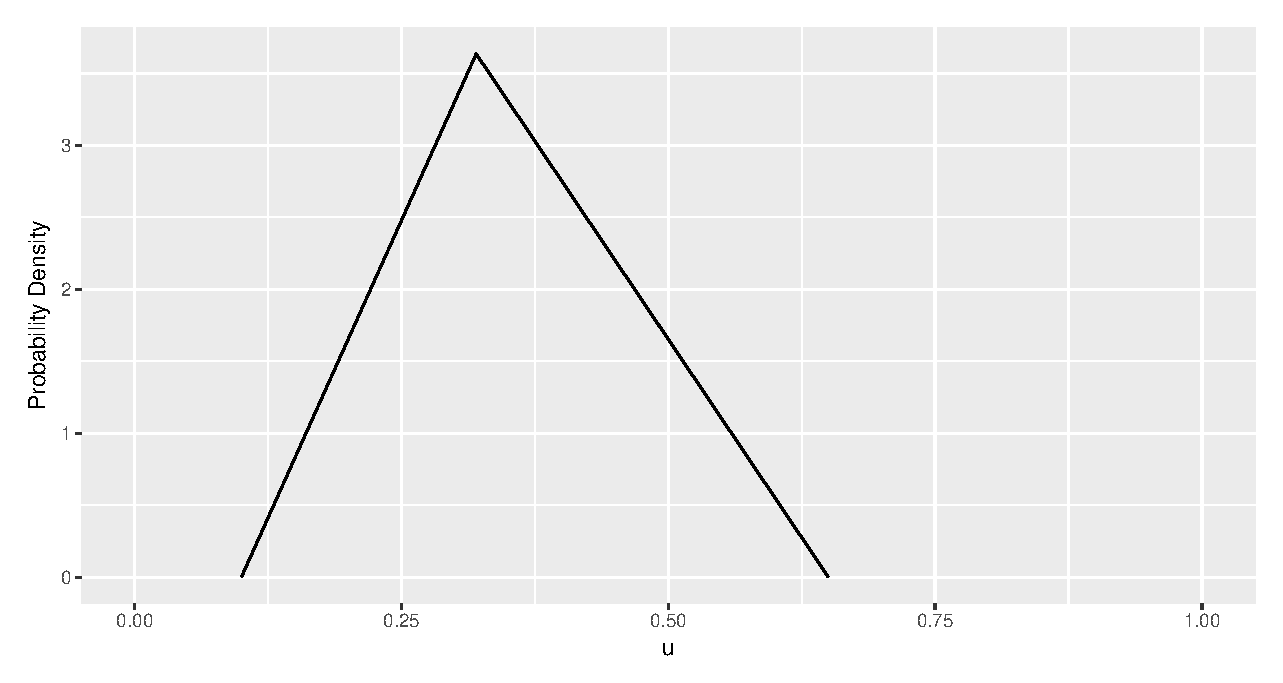
\includegraphics[scale=0.75]{triang.eps}
	\caption{The triangular distribution.}
	\label{triang}
\end{figure}

The gamma distribution is another choice for modelling both the cell size $v$ and the hyperparameter $\lambda$.
Functions for density, distribution function, quantile function and random generation for the gamma distribution  are included in the standard \texttt{R} distribution.

We can assume a parameterization $\Gamma(\alpha + 1, \xi^{*} / \alpha)$, where $\xi^{*}$ stands for the mode of the 
modeled variable ($v$ or $\lambda$) and $\alpha> 0$ determines the degree of concentration 
around the mode $\xi^{*}$ (see figure \ref{gamma}). In the following example we used 5 values for 
$\alpha$, 1, 5, 10, 100, and 1000. The following code shows how to use this distribution.

\begin{verbatim}
alphas <- c(1, 5, 10, 100, 1000)
mode <- 35
df <- lapply(alphas, function(alpha){
    x <- 0:100
    y <- dgamma(x, shape = alpha + 1, scale = mode / alpha)
    z <- as.character(alpha)
    output <- data.frame(x = x, y = y, alpha = z)
    return(output)
})

df <- Reduce(rbind, df)
ggplot(df, aes(x, y, col = alpha, group = alpha)) + 
          geom_line(aes(linetype = alpha)) + 
          scale_x_continuous(limits = c(0, 100)) + xlab('') + ylab('')
\end{verbatim}


\begin{figure}
	\centering
	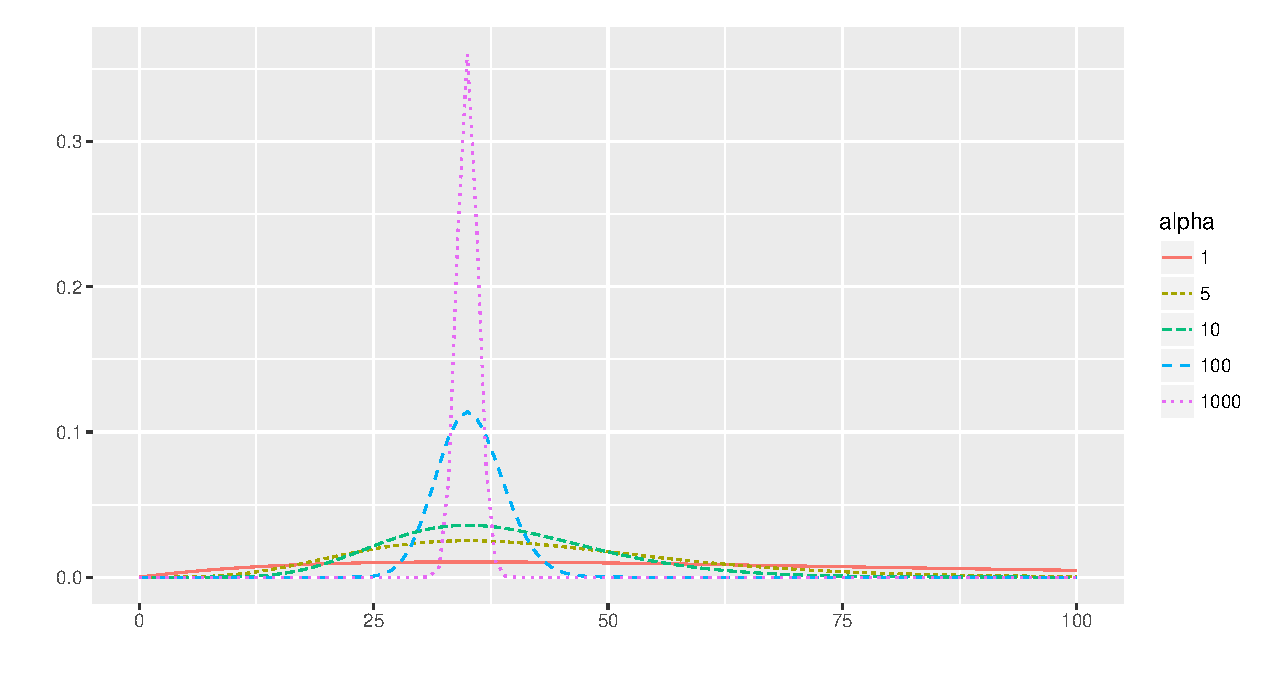
\includegraphics[scale=0.75]{gamma.eps}
	\caption{The gamma distribution.}
	\label{gamma}
\end{figure}


\subsection{Estimation for a single cell}
We can assume that there is a high correlation between the actual size and official population data \cite{Q2016}.
In our examples, for the simulated data that we will generate, for a given actual true 
value $N^{0}_{i}$ we will simulate a population register value $N^{\textrm{REG}_{i}}\simeq \lfloor N(\mu = N^{0}_{i}, \sigma = 10\%\cdot N^{0}_{i})\rfloor$. For the corresponding number of individuals detected through the mobile network we will assume a proportion 
of detected individuals randomly between $15\%$ and $40\%$ as realistic figures (see  \cite{WP5Del11} to compare with market shares as an approximation to these figures).

Since the treatment of all cells is independent of each other, we will start by showing the 
estimation process for a single cell. We investigate different combinations of priors and 
numerical regimes for $N^{\textrm{MNO}}$ and $N^{\textrm{REG}}$. In all cases we assume a 
priori $f_{3}\simeq\Gamma\left(\alpha + 1, \frac{N^{\textrm{Reg}}}{\alpha}\right)$ for $\lambda$.
Let us consider a true population size of $N^{(0)} = 100$, a population given by some administrative register
$N^{\textrm{Reg}}=97$ assuming an error of $3\%$. 
Let us also consider the number of individuals detected by the mobile network as $N^{\textrm{MNO}} = 19$ 
assuming a proportion of detected individuals of around $20\%$.

\subsubsection{$f_{1}\simeq\textrm{Unif}(u_{m}, u_{M})$, $f_{2}\simeq\textrm{triang}(v_{m}, v_{M}, v_{*})$}
For the prior distribution of the proportion 
of detected individuals we will assume a weakly informative distribution 
$f_{u}=\textrm{Unif}(u_{m}, u_{M})$ with $u_{m}=0$ and $u_{M}=0.50$. For the prior 
distribution of the cell size we will assume a triangular distribution with 
parameters $v_{m}=87$, $v_{M}=107$, and $v^{*}=97$, assuming an (unknown) error of $10\%$ over 
the population register size.

Computing the estimates for values of $\alpha=1,10,100,1000$ and observing the effect of the amount of 
uncertainty in the population size (see figure \ref{one}) can be achieved as follows:

\begin{verbatim}
library(pestim)
library(data.table)
library(ggplot2)
nReg <- 97
nMNO <- 19
fu <- list('unif', xMin = 0, xMax = 0.50)
fv <- list('triang', xMin = 87, xMax = 107, xMode = 97)
alphaSeq <- c(1, 10, 100, 1000)
flambdaList <- list()
for (alpha in alphaSeq){
    flambdaList[[as.character(alpha)]] <- 
         list('gamma', shape = 1 + alpha, scale = nReg / alpha)	
}
nSim <- 100
results <- lapply(alphaSeq, function(alpha){
    flambda <- flambdaList[[as.character(alpha)]]
    output <- replicate(nSim, postN0(nMNO, nReg, fu, fv, flambda))
    output <- as.data.table(t(matrix(unlist(output), nrow = 3)))
    setnames(output, c('postMean', 'postMedian', 'postMode'))
    output[, sim := 1:nSim]
    output <- melt(output, id.vars = 'sim')
    output[, 'alpha' := alpha]
    return(output)
})
names(results) <- alphaSeq
results <- rbindlist(results)
ggplot(results, aes(x = variable, y = value)) + 
           geom_boxplot() + facet_grid(. ~ alpha) + 
           xlab('') + ylab('') +  geom_hline(yintercept = nReg) + 
           theme(axis.text.x = element_text(angle = 90, hjust = 1, vjust = .5))
\end{verbatim}

The actual computation of the population estimation is done by \texttt{postN0()} function that takes the following parameters:
\begin{itemize}
\item nMNO - the number of the individuals detected in the actual cell according to the mobile network operator
\item nReg - the number of individuals from the register
\item fu and fv - named lists with the prior marginal distributions of the two-dimensional points for the Monte Carlo integration
\item flambda - named list with the prior distribution of the lambda parameter
\item n - the number of points to generate in the posterior distribution for the computation. Default value is 1e3
\item scale - a numeric vector with the scale to count the number of individuals. Default value is 1
\item relTol - relative tolerance in the computation of the kummer function (default value is 1e-6)
\item nSim - number of two-dimensional points to generate to compute the integral (default value is 1e4)
\item nStrata - integer vector of length 2 with the number of strata in each dimension (default value is c(1, 1e2))
\end{itemize}

In this example we used the default values for \texttt{n, scale, relTol, nSim, nStrata} parameters.

This function generates a $n$ random values for population according to the posterior distribution by calling \texttt{rN0()} function. The posterior distribution used to generates random numbers is a Poisson distribution (see the second row from model  \ref{model1}) . In turn, \texttt{rN0()} calls \texttt{rlambda()} to generate these points. 

\texttt{rlambda()} generates the points according to the accept-reject method using as candidate
distribution a Cauchy distribution whose parameters are taken from the prior distributions and the mode of the posterior distribution of the $\lambda$ parameter as is described at the end of section \ref{model}.
\texttt{rlambda()}  first computes the mode for the posterior distribution of $\lambda$ using \texttt{modeLambda()} function and then apply the acception-rejection method. 
This latter function uses the posterior density function 
of the parameter ${\lambda}$ in the hierarchical model implemented in our package by \texttt{dlambda()}
function. This computes the unnormalized posterior density function of the parameter ${\lambda}$ as 
 ${f(\lambda\big | N^{\textrm{MNO}}; N^{\textrm{Nreg}})\propto f(\lambda)\cdot \textrm{dpois}(N^{\textrm{MNO}}; \lambda)\cdot S(\lambda; N^{\textrm{MNO}}, N^{\textrm{Nreg}}), }$
where \texttt{dpois} is the probability density function of a Poisson distribution and is implemented in the standard \texttt{R} distribution and
$S$ is defined in equation \ref{Sdef1}, \ref{Sdef2}. 

$S$ is computed using the Monte Carlo method described in section \ref{model}. The points needed by this method (see eq.\ref{montecarlo}) are generated using \texttt{genUV()} function and $\Phi$ function from eq. \ref{montecarlo} is evaluated by a call to \texttt{Phi()} 
from \texttt{pestim}. \texttt{Phi()} multiplies a ratio of two $Beta$ functions (eq. \ref{ratioB}) computed by \texttt{ratioBeta()} function and the confluent hypergeometric function which is given by a call to \texttt{kummer()} function. This later function was implemented in C++ and called using \texttt{RCpp} package because it is numerically intensive and the performance of a pure R implementation is far from the C++ implementation in terms of computing time.

We can observe how the more precise the prior value of $\lambda = N^{\textrm{Reg}}$ is, the more precise 
the final estimate around $N^{\textrm{Reg}}$ will result. 
Notice how this final estimate inherits the original difference between $N^{(0)}$ and $N^{\textrm{Reg}}$, as expected.

\begin{figure}
	\centering
	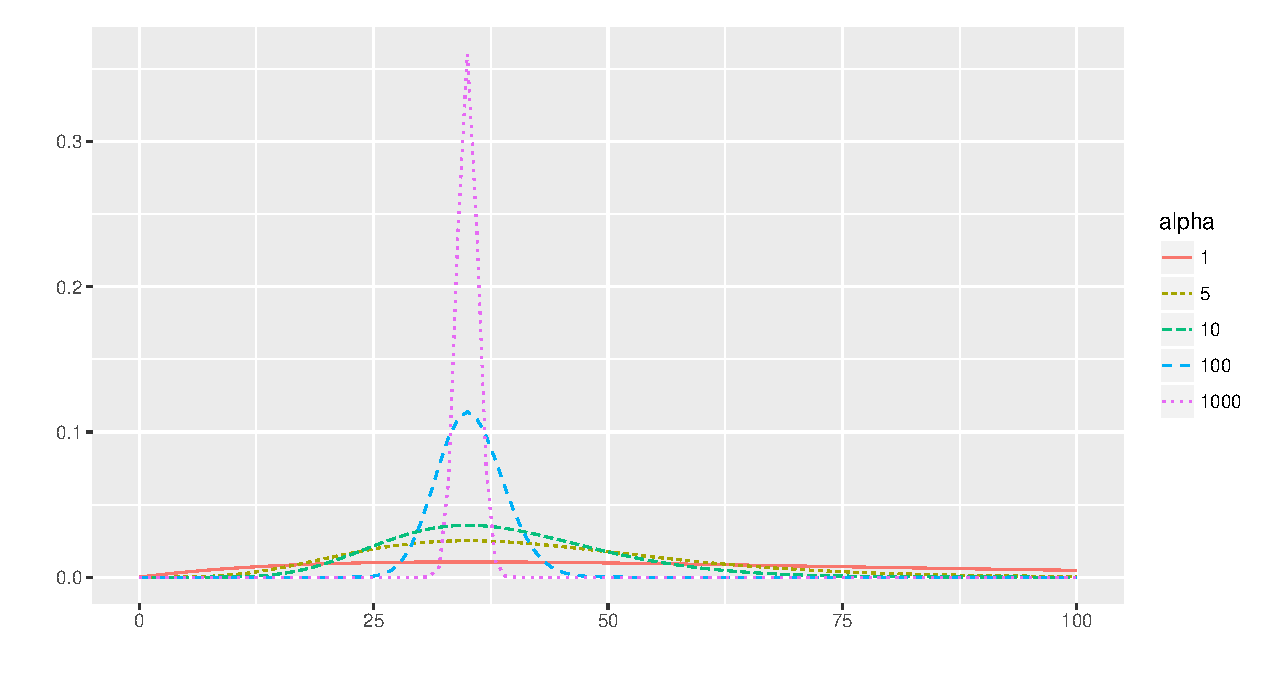
\includegraphics[scale=0.75]{gamma.eps}
	\caption{The uncertainty in population estimation.}
	\label{one}
\end{figure}

\subsubsection{$f_{1}\simeq\textrm{Unif}(u_{m}, u_{M})$, $f_{2}\simeq\textrm{Unif}(N_{m}, N_{M})$}

For the intervals $(u_{m}, u_{M})$ we will choose as centres of the intervals the value $N^{\textrm{MNO}} / N^{\textrm{Reg}}$ and as radii, 
we will progressively shorten the intervals starting from 
$r_{1}=min(N^{\textrm{MNO}} / N^{\textrm{Reg}}, 1- N^{\textrm{MNO}} / N^{\textrm{Reg}})$ down to $0.005$ and we will
use a number of $nPar=10$ points for $u$.

For the intervals $(N_{m}, N_{M})$ we will choose as centres of the intervals the 
natural value $N^{\textrm{Reg}}$ and as radii, we will progressively shorten the intervals starting from 
$R_{1}=\lfloor 0.25\cdot N^{\textrm{Reg}}\rfloor$ down to $1$ and we will also use the same number $nPar=10$ of points.

In all cases we will use $\alpha = 1$ as a weakly informative choice. For each pair of 
interval lengths $(u_{M}-u_{m}, N_{M} - N_{m})$ we will estimate the population and compute the relative
bias $\frac{\hat{N}-N^{\textrm{Reg}}}{N^{\textrm{Reg}}} \cdot 100$ for 
the posterior mean, median and mode estimates. The following piece of code does this estimation (to keep
the length of this document reasonable we don't reproduce here the actual numerical results).
One can note that this code is similar with the previous example, the estimation being computed with a call to \texttt{postN0()} function, and only the prior distributions are different.

\begin{verbatim}
library(pestim)
library(data.table)
nReg <- 97
nMNO <- 19
nPar <- 10
radShares <- seq(from = nMNO / nReg, to = 0.005, length.out = nPar)
radPopSizes <- round(seq(from = 0.25 * nReg, to = 1, length.out = nPar))
alpha <- 1
flambda <- list('gamma', shape = alpha + 1, scale = nReg / alpha)
results.Mean <- matrix(NA, ncol = nPar, nrow = nPar)
results.Median <- matrix(NA, ncol = nPar, nrow = nPar)
results.Mode <- matrix(NA, ncol = nPar, nrow = nPar)
for (radShare.index in seq(along = radShares)) {
    for (radPopSize.index in seq(along = radPopSizes)) {
        um <- nMNO / nReg - radShares[radShare.index]
        uM <- nMNO / nReg + radShares[radShare.index]
        fu <- list('unif', xMin = um, xMax = uM)
        Nm <- nReg - radPopSizes[radPopSize.index]
        NM <- nReg + radPopSizes[radPopSize.index]
        fv <- list('unif', xMin = Nm, xMax = NM)
        auxResults <- postN0(nMNO, nReg, fu, fv, flambda)
        results.Mean[radShare.index, radPopSize.index] <- auxResults[['postMean']] 
        results.Median[radShare.index, radPopSize.index] <- auxResults[['postMedian']]
        results.Mode[radShare.index, radPopSize.index] <- auxResults[['postMode']]
        }
}
rownames(results.Mean) <- round(2 * radShares, 2)
rownames(results.Median) <- round(2 * radShares, 2)
rownames(results.Mode) <- round(2 * radShares, 2)
colnames(results.Mean) <- 2 * radPopSizes
colnames(results.Median) <- 2 * radPopSizes
colnames(results.Mode) <- 2 * radPopSizes
relBias.Mean <- round((results.Mean - nReg) / nReg * 100, 1)
relBias.Median <- round((results.Median - nReg) / nReg * 100, 1)
relBias.Mode <- round((results.Mode - nReg) / nReg * 100, 1)
\end{verbatim}

\subsubsection{$f_{1}\simeq\textrm{Unif}(u_{m}, u_{M})$, $f_{2}\simeq\textrm{triang}(N_{m}, N_{M}, N^{\textrm{Reg}})$}

The same computations as in the preceding section is carried out using a triangular prior distribution $f_{2}$ for the actual
population size. The limits $N_{m}$ and $N_{M}$ are chosen as in the preceding section and the mode as $N^{*}=N^{\textrm{Reg}}$.

\begin{verbatim}
library(pestim)
library(data.table)
nReg <- 97
nMNO <- 19
nPar <- 10
radShares <- seq(from = nMNO / nReg, to = 0.005, length.out = nPar)
radPopSizes <- round(seq(from = 0.25 * nReg, to = 1, length.out = nPar))
alpha <- 1
flambda <- list('gamma', shape = alpha + 1, scale = nReg / alpha)
results.Mean <- matrix(NA, ncol = nPar, nrow = nPar)
results.Median <- matrix(NA, ncol = nPar, nrow = nPar)
results.Mode <- matrix(NA, ncol = nPar, nrow = nPar)
for (radShare.index in seq(along = radShares)) {
    for (radPopSize.index in seq(along = radPopSizes)) {
        um <- nMNO / nReg - radShares[radShare.index]
        uM <- nMNO / nReg + radShares[radShare.index]
        fu <- list('unif', xMin = um, xMax = uM)
        Nm <- nReg - radPopSizes[radPopSize.index]
        NM <- nReg + radPopSizes[radPopSize.index]
        fv <- list('triang', xMin = Nm, xMax = NM, xMode = nReg)
        auxResults <- postN0(nMNO, nReg, fu, fv, flambda)
        results.Mean[radShare.index, radPopSize.index] <- auxResults[['postMean']] 
        results.Median[radShare.index, radPopSize.index] <- auxResults[['postMedian']]
        results.Mode[radShare.index, radPopSize.index] <- auxResults[['postMode']]
    }
}
rownames(results.Mean) <- round(2 * radShares, 2)
rownames(results.Median) <- round(2 * radShares, 2)
rownames(results.Mode) <- round(2 * radShares, 2)
colnames(results.Mean) <- 2 * radPopSizes
colnames(results.Median) <- 2 * radPopSizes
colnames(results.Mode) <- 2 * radPopSizes
relBias.Mean <- round((results.Mean - nReg) / nReg * 100, 1)
relBias.Median <- round((results.Median - nReg) / nReg * 100, 1)
relBias.Mode <- round((results.Mode - nReg) / nReg * 100, 1)
\end{verbatim}

\subsubsection{$f_{1}\simeq\textrm{Unif}(u_{m}, u_{M})$, $f_{2}\simeq\Gamma(a + 1, \frac{N^{\textrm{Reg}}}{a})$}

The same computation is exemplified now with $f_{2}\simeq\Gamma(a+1, \frac{N^{\textrm{Reg}}}{a})$ and $\log_{10}(a)=-3, -2, \dots, 2, 3$.


\begin{verbatim}
library(pestim)
library(data.table)
nReg <- 97
nMNO <- 19
nPar <- 10
radShares <- seq(from = nMNO / nReg, to = 0.005, length.out = nPar)
aPopSizes <- 10^{seq(-3, 3, by = 1)}
alpha <- 1
flambda <- list('gamma', shape = alpha + 1, scale = nReg / alpha)
results.Mean <- matrix(NA, ncol = length(aPopSizes), nrow = length(radShares))
results.Median <- matrix(NA, ncol = length(aPopSizes), nrow = length(radShares))
results.Mode <- matrix(NA, ncol = length(aPopSizes), nrow = length(radShares))
for(radShare.index in seq(along = radShares)) {
    um <- nMNO / nReg - radShares[radShare.index]
    uM <- nMNO / nReg + radShares[radShare.index]
    fu <- list('unif', xMin = um, xMax = uM)
    for (aPopSize.index in seq(along = aPopSizes)) {
        fv <- list('gamma', shape = aPopSizes[aPopSize.index], 
                 scale = nReg / aPopSizes[aPopSize.index])
        auxResults <- postN0(nMNO, nReg, fu, fv, flambda)
        results.Mean[radShare.index, aPopSize.index] <- auxResults[['postMean']] 
        results.Median[radShare.index, aPopSize.index] <- auxResults[['postMedian']]
        results.Mode[radShare.index, aPopSize.index] <- auxResults[['postMode']]
    }
}
rownames(results.Mean) <- round(2 * radShares, 2)
rownames(results.Median) <- round(2 * radShares, 2)
rownames(results.Mode) <- round(2 * radShares, 2)
colnames(results.Mean) <- aPopSizes
colnames(results.Median) <- aPopSizes
colnames(results.Mode) <- aPopSizes
relBias.Mean <- round((results.Mean - nReg) / nReg * 100, 1)
relBias.Median <- round((results.Median - nReg) / nReg * 100, 1)
relBias.Mode <- round((results.Mode - nReg) / nReg * 100, 1)
\end{verbatim}

\subsubsection{$f_{1}\simeq\textrm{Triang}(u_{m}, u_{M}, u^{*})$, $f_{2}\simeq\textrm{Unif}(N_{m}, N_{M})$}

The same example is shown now for $f_{1}\simeq\textrm{Triang}$ and $f_{2}\simeq\textrm{Unif}$. The hyperparameters are chosen as before.

\begin{verbatim}
library(pestim)
library(data.table)
nReg <- 97
nMNO <- 19
nPar <- 10
radShares <- seq(from = nMNO / nReg, to = 0.005, length.out = nPar)
radPopSizes <- round(seq(from = 0.25 * nReg, to = 1, length.out = nPar))
alpha <- 1
flambda <- list('gamma', shape = alpha + 1, scale = nReg / alpha)
results.Mean <- matrix(NA, ncol = nPar, nrow = nPar)
results.Median <- matrix(NA, ncol = nPar, nrow = nPar)
results.Mode <- matrix(NA, ncol = nPar, nrow = nPar)
for(radShare.index in seq(along = radShares)) {
    um <- nMNO / nReg - radShares[radShare.index]
    uM <- nMNO / nReg + radShares[radShare.index]
    uMode <- nMNO / nReg
    fu <- list('triang', xMin = um, xMax = uM, xMode = uMode)
    for(radPopSize.index in seq(along = radPopSizes)) {
        Nm <- nReg - radPopSizes[radPopSize.index]
        NM <- nReg + radPopSizes[radPopSize.index]
        fv <- list('unif', xMin = Nm, xMax = NM)
        auxResults <- postN0(nMNO, nReg, fu, fv, flambda)
        results.Mean[radShare.index, radPopSize.index] <- auxResults[['postMean']] 
        results.Median[radShare.index, radPopSize.index] <- auxResults[['postMedian']]
        results.Mode[radShare.index, radPopSize.index] <- auxResults[['postMode']]
    }
}
rownames(results.Mean) <- round(2 * radShares, 2)
rownames(results.Median) <- round(2 * radShares, 2)
rownames(results.Mode) <- round(2 * radShares, 2)
colnames(results.Mean) <- 2 * radPopSizes
colnames(results.Median) <- 2 * radPopSizes
colnames(results.Mode) <- 2 * radPopSizes
relBias.Mean <- round((results.Mean - nReg) / nReg * 100, 1)
relBias.Median <- round((results.Median - nReg) / nReg * 100, 1)
relBias.Mode <- round((results.Mode - nReg) / nReg * 100, 1)
\end{verbatim}


\subsubsection{$f_{1}\simeq\textrm{Triang}(u_{m}, u_{M}, u^{*})$, $f_{2}\simeq\textrm{Triang}(N_{m}, N_{M}, N^{\textrm{Reg}})$}

Both prior distributions are considered too be traingular with the same choice for hyperparameters.

\begin{verbatim}
library(pestim)
library(data.table)
nReg <- 97
nMNO <- 19
nPar <- 10
radShares <- seq(from = nMNO / nReg, to = 0.005, length.out = nPar)
radPopSizes <- round(seq(from = 0.25 * nReg, to = 1, length.out = nPar))
alpha <- 1
flambda <- list('gamma', shape = alpha + 1, scale = nReg / alpha)
results.Mean <- matrix(NA, ncol = nPar, nrow = nPar)
results.Median <- matrix(NA, ncol = nPar, nrow = nPar)
results.Mode <- matrix(NA, ncol = nPar, nrow = nPar)
for(radShare.index in seq(along = radShares)) {
    um <- nMNO / nReg - radShares[radShare.index]
    uM <- nMNO / nReg + radShares[radShare.index]
    uMode <- nMNO / nReg
    fu <- list('triang', xMin = um, xMax = uM, xMode = uMode)
    for(radPopSize.index in seq(along = radPopSizes)) {
        Nm <- nReg - radPopSizes[radPopSize.index]
        NM <- nReg + radPopSizes[radPopSize.index]
        Nmode <- nReg
        fv <- list('triang', xMin = Nm, xMax = NM, xMode = nReg)
        auxResults <- postN0(nMNO, nReg, fu, fv, flambda)
        results.Mean[radShare.index, radPopSize.index] <- auxResults[['postMean']] 
        results.Median[radShare.index, radPopSize.index] <- auxResults[['postMedian']]
        results.Mode[radShare.index, radPopSize.index] <- auxResults[['postMode']]
    }
}
rownames(results.Mean) <- round(2 * radShares, 2)
rownames(results.Median) <- round(2 * radShares, 2)
rownames(results.Mode) <- round(2 * radShares, 2)
colnames(results.Mean) <- 2 * radPopSizes
colnames(results.Median) <- 2 * radPopSizes
colnames(results.Mode) <- 2 * radPopSizes
relBias.Mean <- round((results.Mean - nReg) / nReg * 100, 1)
relBias.Median <- round((results.Median - nReg) / nReg * 100, 1)
relBias.Mode <- round((results.Mode - nReg) / nReg * 100, 1)
\end{verbatim}

\subsubsection{$f_{1}\simeq\textrm{Triang}(u_{m}, u_{M}, u^{*})$, $f_{2}\simeq\Gamma(a + 1, \frac{N^{\textrm{Reg}}}{a})$}

In the last example we combined a triangular distribution for $f_{1}$ and a gamma distribution for $f_{2}$.
\begin{verbatim}
library(pestim)
library(data.table)
nReg <- 97
nMNO <- 19
nPar <- 10
radShares <- seq(from = nMNO / nReg, to = 0.005, length.out = nPar)
aPopSizes <- 10^{seq(-3, 3, by = 1)}
alpha <- 1
flambda <- list('gamma', shape = alpha + 1, scale = nReg / alpha)
results.Mean <- matrix(NA, ncol = length(aPopSizes), nrow = length(radShares))
results.Median <- matrix(NA, ncol = length(aPopSizes), nrow = length(radShares))
results.Mode <- matrix(NA, ncol = length(aPopSizes), nrow = length(radShares))
for(radShare.index in seq(along = radShares)) {
    um <- nMNO / nReg - radShares[radShare.index]
    uM <- nMNO / nReg + radShares[radShare.index]
    uMode <- nMNO / nReg
    fu <- list('triang', xMin = um, xMax = uM, xMode = uMode)
    for(aPopSize.index in seq(along = aPopSizes)) {
        fv <- list('gamma', shape = aPopSizes[aPopSize.index], 
                       scale = nReg / aPopSizes[aPopSize.index])
        auxResults <- postN0(nMNO, nReg, fu, fv, flambda)
        results.Mean[radShare.index, aPopSize.index] <- auxResults[['postMean']] 
        results.Median[radShare.index, aPopSize.index] <- auxResults[['postMedian']]
        results.Mode[radShare.index, aPopSize.index ] <- auxResults[['postMode']]
    }
}
rownames(results.Mean) <- round(2 * radShares, 2)
rownames(results.Median) <- round(2 * radShares, 2)
rownames(results.Mode) <- round(2 * radShares, 2)
colnames(results.Mean) <- aPopSizes
colnames(results.Median) <- aPopSizes
colnames(results.Mode) <- aPopSizes
relBias.Mean <- round((results.Mean - nReg) / nReg * 100, 1)
relBias.Median <- round((results.Median - nReg) / nReg * 100, 1)
relBias.Mode <- round((results.Mode - nReg) / nReg * 100, 1)
\end{verbatim}


\subsection{Estimation for several cells}

Obtaining estimations for the target population for a grid of cells is similar to the process for a single cell since the estimation in each cell is independent of each other.

We can consider the ratios $\frac{N_{i}^{\textrm{MNO}}}{N^{\textrm{Reg}}_{i}}$ 
as an initial guess for the proportions of detected individuals $u_{i}$ 
with a highly probable value whose uncertainty will depend both on the process to obtain $N_{i}^{\textrm{MNO}}$ 
(preprocessing and aggregation stages of the mobile phone data) 
and on the process to compile the population register figures $N_{i}^{\textrm{Reg}}$ 
(measurement errors, processing errors, coverage, etc.). 
Any of the three prior distributions (uniform, triangular, gamma) can be used to express this 
uncertainty around $\frac{N_{i}^{\textrm{MNO}}}{N^{\textrm{Reg}}_{i}}$. 

For the prior distribution for the local cell size $v_{i}$ we can make similar 
considerations around the value $N_{i}^{\textrm{Reg}}$ for each cell $i$ focusing on the 
process of construction of the population register.

The prior distribution for the parameter $\lambda_{i}$ is very important. 
If we choose $\alpha_{i}\gg 1$, this means a high confidence on 
the population register as the true population. It is advisable to be conservative 
and choose low values so that we do not artificially  \textquotedblleft force\textquotedblright\ 
the final estimates to be close to $N_{i}^{\textrm{Reg}}$. In the choice of $\alpha_{i}$ we can make use of the grid construction and the distribution 
of $N_{i}^{\textrm{Reg}}$ to propose some prior values. 

The variance of $\Gamma(\alpha_{i} + 1, \frac{N^{\textrm{Reg}}_{i}}{\alpha_{i}})$ 
is $\frac{\alpha_{i} + 1}{\alpha_{i}^{2}}\cdot N^{\textrm{Reg}}_{i}$ and under the 
assumption of having a regular grid over the population, we can equate 
$\frac{\alpha_{i} + 1}{\alpha_{i}^{2}}\cdot N^{\textrm{Reg}}=\frac{1}{N_{cells} - 1}\sum_{i=1}^{N_{cell}}\left(N_{i}^{\textrm{Reg}} - \bar{N}^{\textrm{Reg}}\right)^{2}$
to have a first value (upper bound) for $\alpha\leq\min_{i}\alpha_{i}$. 

The estimation processes for the prior hyperparameters are very important if we want to obtain final estimates not based upon subjective beliefs.

In the following we will show an example how to estimate the population in $N_{c}=50$ cells, 
and we will consider a range of values for the hyperparameters to observe the effects on the final estimate.
For the intervals $(u_{m,i}, u_{M,i})$ we will choose as centres of the intervals the 
natural values $N^{\textrm{MNO}}_{i} / N^{\textrm{Reg}}_{i}$ and as radii, we will progressively 
shorten the intervals starting from $r_{1,i}=min(N^{\textrm{MNO}}_{i} / N^{\textrm{Reg}}_{i}, 1- N^{\textrm{MNO}}_{i} / N^{\textrm{Reg}}_{i})$ down to $0.005$.
For the intervals $(N_{m,i}, N_{M,i})$ we will choose as centres of the intervals the natural 
values $N^{\textrm{Reg}}_{i}$ and as radii, we will progressively shorten the intervals starting 
from $R_{1,i}=\lfloor 0.25\cdot N^{\textrm{Reg}}_{i}\rfloor$ down to $1$. We will generate a number
of $nPar=5$ values for each interval.

The following piece of code computes and displays the distribution of the relative 
bias $\frac{\hat{N}_{i}-N^{\textrm{Reg}}_{i}}{N^{\textrm{Reg}}} \cdot 100$ for the posterior mean, median and mode estimates, respectively, 
for all pairs of interval lengths $(u_{M,i}-u_{m,i}, N_{M,i} - N_{m,i})$ and all cells. The values for posterior distribution of the population is again obtained by a call to \texttt{postNo()} function. 

\begin{verbatim}
library(pestim)
library(data.table)
library(ggplot2)
nCell <- 50
nReg <- round(rnorm(nCell, 71, 3))
nMNO <- round(rnorm(nCell, 19, 2))
nPar <- 5
radShares <- lapply(1:nCell, function(i){
    seq(from = (nMNO / nReg)[i], to = 0.005, length.out = nPar)
})
radPopSizes <- lapply(1:nCell, function(i){
    round(seq(from = 0.25 * nReg[i], to = 1, length.out = nPar))
})
varnReg <- var(nReg)
alphaBound <- sapply(1:nCell, function(i){
    0.5 * (nReg[i] / varnReg + sqrt((nReg[i] / varnReg)^2 + 4 * nReg[i] / varnReg))
})
alpha <- min(alphaBound)
results.Mean <- lapply(1:nCell, function(i){matrix(NA, ncol = nPar, nrow = nPar)})
results.Median <- lapply(1:nCell, function(i){matrix(NA, ncol = nPar, nrow = nPar)})
results.Mode <- lapply(1:nCell, function(i){matrix(NA, ncol = nPar, nrow = nPar)})
relBias.Mean <- list()
relBias.Median <- list()
relBias.Mode <- list()
for(i in 1:nCell){
    for(radShare.index in seq(along = radShares[[i]])) {
        for (radPopSize.index in seq(along = radPopSizes[[i]])) {
            um <- nMNO[[i]] / nReg[[i]] - radShares[[i]][radShare.index]
            uM <- nMNO[[i]] / nReg[[i]] + radShares[[i]][radShare.index]
            fu <- list('unif', xMin = um, xMax = uM)
            Nm <- nReg[[i]] - radPopSizes[[i]][radPopSize.index]
            NM <- nReg[[i]] + radPopSizes[[i]][radPopSize.index]
            fv <- list('unif', xMin = Nm, xMax = NM)
            flambda <- list('gamma', shape = alpha + 1, scale = nReg[[i]] / alpha)
            auxResults <- postN0(nMNO[[i]], nReg[[i]], fu, fv, flambda)
            results.Mean[[i]][radShare.index, radPopSize.index] <- 
                    auxResults[['postMean']] 
            results.Median[[i]][radShare.index, radPopSize.index] <- 
                    auxResults[['postMedian']]
            results.Mode[[i]][radShare.index, radPopSize.index] <- 
                    auxResults[['postMode']]
        }
    }
    rownames(results.Mean[[i]]) <- round(2 * radShares[[i]], 2)
    rownames(results.Median[[i]]) <- round(2 * radShares[[i]], 2)
    rownames(results.Mode[[i]]) <- round(2 * radShares[[i]], 2)
    colnames(results.Mean[[i]]) <- 2 * radPopSizes[[i]]
    colnames(results.Median[[i]]) <- 2 * radPopSizes[[i]]
    colnames(results.Mode[[i]]) <- 2 * radPopSizes[[i]]
    relBias.Mean[[i]] <- 
               round((results.Mean[[i]] - nReg[[i]]) / nReg[[i]] * 100, 1)
    relBias.Median[[i]] <- 
               round((results.Median[[i]] - nReg[[i]]) / nReg[[i]] * 100, 1)
    relBias.Mode[[i]] <- 
               round((results.Mode[[i]] - nReg[[i]]) / nReg[[i]] * 100, 1)
}
parNames <- expand.grid(paste0('u', 1:5), paste0('v', 1:5))
colnames(parNames) <- c('u', 'v')

relBias.Mean.df <- 
           data.frame(u = character(0), v = character(0), 
           cell = character(0), N = numeric(0))
relBias.Median.df <- 
           data.frame(u = character(0), v = character(0), 
           cell = character(0), N = numeric(0))
relBias.Mode.df <- 
           data.frame(u = character(0), v = character(0), 
           cell = character(0), N = numeric(0))
for(i in 1:nCell){
    aux <- cbind(parNames, cell = as.character(i), N = as.vector(relBias.Mean[[i]]))
    relBias.Mean.df <- rbind(relBias.Mean.df, aux)
    aux <- cbind(parNames, cell = as.character(i), N = as.vector(relBias.Median[[i]]))
    relBias.Median.df <- rbind(relBias.Median.df, aux)
    aux <- cbind(parNames, cell = as.character(i), N = as.vector(relBias.Mode[[i]]))
    relBias.Mode.df <- rbind(relBias.Mode.df, aux)
}
ggplot(relBias.Mean.df, aes(x = ' ', y = N)) + geom_boxplot() +
            facet_grid(factor(u) ~ factor(v)) + 
            xlab('Diverse combinations of prior parameters') + 
            ylab('Mean Estimates\n') +
            ggtitle(paste0('Relative bias (%) distributions of the ', 
            nCell, ' cells\n')) +
            theme(plot.title = element_text(face = 'bold', size = 14, hjust = 0.5))

ggplot(relBias.Median.df, aes(x = ' ', y = N)) + geom_boxplot() +
           facet_grid(factor(u) ~ factor(v)) +
           xlab('Diverse combinations of prior parameters') + 
           ylab('Median Estimates\n') +
           ggtitle(paste0('Relative bias (%) distributions of the ', 
           nCell, ' cells\n')) +
           theme(plot.title = element_text(face = 'bold', size = 14, hjust = 0.5))

ggplot(relBias.Mode.df, aes(x = ' ', y = N)) + geom_boxplot() +
           facet_grid(factor(u) ~ factor(v)) +
           xlab('Diverse combinations of prior parameters') + 
           ylab('Mode Estimates\n') +
           ggtitle(paste0('Relative bias (%) distributions of the ', 
           nCell, ' cells\n')) +
           theme(plot.title = element_text(face = 'bold', size = 14, hjust = 0.5))
\end{verbatim}

The same combinations for distributions used for $f_{1}$ and $f_{2}$ can be done in the case of several cell like in  the case of a single cell. Since this process is straightforward we will not show here each combination.


\section{Estimates along a sequence of time}

In this section we show how to extend the previous estimates along a sequence of time instants. This process is represented in figure \ref{Tool2}.

\begin{figure}[htbp]
	\centering
	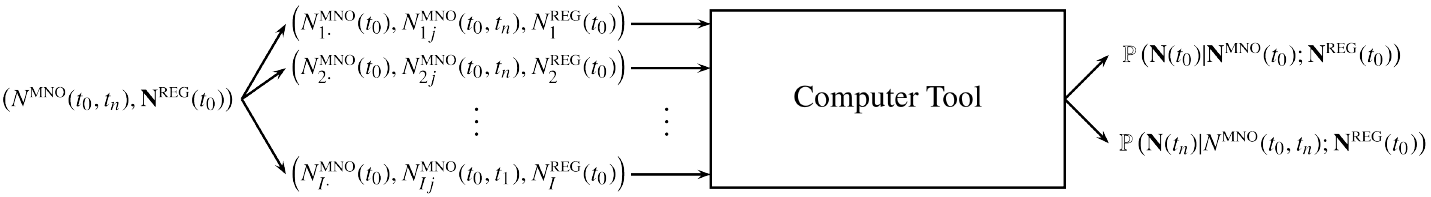
\includegraphics[scale=0.35]{Tool2.png}
	\caption{A diagram of the estimation process for the target population using mobile phone and official population data at a sequence of time instants.}
	\label{Tool2} 
\end{figure}

As input data for the final inference stage we used the number of individuals $N_{ij}^{\textrm{MNO}}(t_{0}, t_{n})$ moving from territorial cell $i$ to cell $j$ in the time interval $(t_{0}, t_{n})$ according to the MNO. These data will be combined with official data and at the end we will  provide the following outputs:

\begin{itemize}
	\item the probability distribution of actual individuals in each territorial cell $i$ at the initial time $t_{0}$;
	\item the probability distribution of actual individuals at the time instants $t_{n}$ for $n=1,2,\dots$.
\end{itemize}  

We make two prior assumptions:

\begin{enumerate}
	\item To combine both aggregated mobile phone and official data we assume that a given time instant $t_{0}$ both population figures in each territorial cell can be equated to some extent. For simplicity we will take $N_{i}^{\textrm{Reg}}$ as a fixed quantity without a prior distribution representing uncertainty in its knowledge. Therefore $N_{i}^{\textrm{Reg}}$ will be fixed external parameters in the model. 
	\item The movements of individuals from one cell to another cell is assumed to be independent of being subscribers of a given MNO or another.
\end{enumerate}

The following hierchical model supports these hypotheses. Let $p_{ij}(t_{0}, t_{n})$ denote the probability for an individual to move from cell $i$ to cell $j$ in the time interval $(t_{0}, t_{n})$. Let $N_{ij}^{\textrm{MNO}}(t_{0}, t_{n})$ the number of individuals moving from cell $i$ to cell $j$ according to the network. We denote $N_{i\cdot}^{\textrm{MNO}}(t_{0})=\sum_{j=1}^{I}N_{ij}^{\textrm{MNO}}(t_{0}, t_{n})$. 

\begin{subequations}
	\begin{align}
	\label{eq:Model2Ini}N_{i}(t_{n}) & = \left[ N_{i}(t_{0}) + \sum_{\substack{j=1\\j\neq i}}^{I}p_{ji}(t_{0}, t_{n})N_{j}(t_{0})-\sum_{\substack{j=1\\j\neq i}}^{I}p_{ij}(t_{0}, t_{n}) N_{i}(t_{0})\right ],\quad i=1,\dots,I\\ 
	\label{eq:Model2Mid}\mathbf{p}_{i\cdot}(t_{0}, t_{n})& \simeq\textrm{Dir}\left(\alpha_{i1}(t_{0}, t_{n}), \dots, \alpha_{iI}(t_{0}, t_{n})\right),\quad \mathbf{p}_{i\cdot}(t_{0}, t_{n})\perp\mathbf{p}_{j\cdot}(t_{0}, t_{n}),\quad i\neq j=1,\dots,I\\
	\label{eq:Model2Fin}\alpha_{ij}(t_{0}, t_{n})&\simeq f_{\alpha ij}\left(\alpha_{ij}; \frac{N_{ij}^{\textrm{MNO}}(t_{0}, t_{n})}{N_{i\cdot}^{\textrm{MNO}}(t_{0})}\right), \quad i=1,\dots,I\\
	\label{eq:Model1Ini}N_{i}^{\textrm{MNO}}(t_{0})&\simeq\textrm{Bin}\left(N_{i}(t_{0}), p_{i}(t_{0})\right),\qquad N_{i}^{\textrm{MNO}}(t_{0})\perp N_{j}^{\textrm{MNO}}(t_{0}),\quad i\neq j=1,\dots,I\\
	N_{i}(t_{0})&\simeq\textrm{Po}\left(\lambda_{i}(t_{0})\right),\qquad N_{i}(t_{0})\perp N_{j}(t_{0}),\quad i\neq j=1,\dots,I\\
	p_{i}(t_{0})&\simeq\textrm{Beta}\left(\alpha_{i}(t_{0}),\beta_{i}(t_{0})\right),\qquad p_{i}(t_{0})\perp p_{j}(t_{0})\quad i\neq j=1,\dots,I\\
	\left(\alpha_{i}(t_{0}), \beta_{i}(t_{0})\right)&\simeq \frac{f_{ui}\left(\frac{\alpha_{i}}{\alpha_{i}+\beta_{i}}; \frac{N_{i}^{\textrm{MNO}}(t_{0})}{N_{i}^{\textrm{REG}}(t_{0})}\right)\cdot f_{vi}\left(\alpha_{i}+\beta_{i}; N_{i}^{\textrm{REG}}(t_{0})\right)}{\alpha_{i}+\beta_{i}},\nonumber \\ &(\alpha_{i}(t_{0}),\beta_{i}(t_{0}))\perp(\alpha_{j}(t_{0}),\beta_{j}(t_{0})),\quad i\neq j=1,\dots,I\\
	\label{eq:Model1Fin}\lambda_{i}(t_{0})&\simeq f_{\lambda i}(\lambda_{i}; N_{i}^{\textrm{REG}}(t_{0}))\quad (\lambda_{i}(t_{0}) > 0,\quad \lambda_{i}(t_{0})\perp\lambda_{j}(t_{0})), \quad i=1,\dots,I,
	\end{align}
\end{subequations}

\noindent where 

\begin{itemize}
	\item $[\cdot]$ denotes the nearest integer function;
	\item $f_{\alpha ij}$ is the probability density function of the parameters $\alpha_{ij}$. The notation $f_{\alpha ij}\left(\alpha_{ij}; \frac{N_{ij}^{\textrm{MNO}}(t_{0}, t_{n})}{N_{i\cdot}^{\textrm{MNO}}(t_{0})}\right)$ is meant to indicate that $\frac{N_{ij}^{\textrm{MNO}}(t_{0}, t_{n})}{N_{i\cdot}^{\textrm{MNO}}(t_{0})}$ should be taken as the mode of the density function;
	\item $f_{ui}$ is the probability density function of the parameter $u$ in cell $i$ with mode $\frac{N_{i}^{\textrm{MNO}}(t_{0})}{N_{i}^{\textrm{REG}}(t_{0})}$;
	\item $f_{vi}$ isr the probability density function of the parameter $v$  in cell $i$ with mode $N_{i}^{\textrm{REG}}(t_{0})$;
	\item $f_{\lambda i}$ is the probability density function of the parameter $\lambda$ in cell $i$ with mode $N_{i}^{\textrm{REG}}(t_{0})$. 
\end{itemize}


Equations \eqref{eq:Model1Ini} to \eqref{eq:Model1Fin} add time dependence to the model described in section \ref{model}. Equations \eqref{eq:Model2Ini}, \eqref{eq:Model2Mid}, \eqref{eq:Model2Fin} take care of the time evolution of the estimates.

Equation \eqref{eq:Model2Ini} states that the number of individuals in a cell $i$ at time $t_{n}$ equals the initial number of individuals plus those arriving from other cells in the given time interval minus those leaving for other cells in the same time interval. The number of individuals arriving and leaving are estimated using the transition probability among cells.

We modelled these transition probabilities for a given cell $i$ as a multivariate random variable with a Dirichlet distribution with parameters $\alpha_{i1},\dots,\alpha_{iI}$. These parameters  are given unimodal prior distributions $f_{\alpha_{ij}}$ with mode in $\frac{N_{ij}^{\textrm{MNO}}}{N_{i\cdot}^{\textrm{MNO}}}$ according to our second working assumption.

The computation of the probability functions $\mathbb{P}\left(N_{i}(t_{n})\big|N^{\textrm{MNO}}(t_{0}, t_{1})\right)$ for each cell $i$ will allow us to choose an estimator as, e.g., the posterior mean, posterior median or posterior mode. The computation is conducted empirically in three steps:

\begin{enumerate}
	\item The initial population value $N_{i}(t_{0})$ is generated for all cells $i=1,\dots, I$ according to the model using $N_{i\cdot}^{\textrm{MNO}}(t_{0})$ as input data and choosing weakly informative priors $f_{ui}$, $f_{vi}$ and $f_{\lambda i}$.
	\item A transition probability matrix $[p_{ij}(t_{0}, t_{n})]$ is generated according to the model using $N^{\textrm{MNO}}(t_{0}, t_{n})$ as input data and choosing weakly informative priors $f_{\alpha ij}$.
	\item These generated quantities are used in formula \eqref{eq:Model2Ini} to generate $N_{i}(t_{1})$ for all cells $i=1,\dots,I$.
\end{enumerate}

Following these steps we can generate an empirical posterior distribution of values $N_{i}(t_{n})$ for each cell $i$. Then we can use these distributions to provide a point estimate according to its mean, median, or mode.


\section{An example how to estimate population at a sequence of time instants}

In this example we will consider a territory divided into $12$ cells. At $4$ succesive time intervals the individuals follow their own trajectories so that the population in each cell evolves according to actual transition matrices $N_{ij}(t_{n-1}, t_{n})$, $n=1,2,3,4$. At the initial time instant $t_{0}$ we also have the population register figures for each cell $N_{i}^{\textrm{Reg}}(t_{0})$ which can be equated to the initial real population $N_{i}(t_{0})$, although they are not completely equal due to nonsampling errors.

We also generate the transition matrices for each time interval $n=1,2,3,4$ for the individuals $N_{ij}^{\textrm{MNO}}(t_{n-1}, t_{n})$ detected with the network.

\texttt{pestim} contains a dataset \texttt{MobPop} that provides population counts moving from 
each pair of cells at succesive time instants for a simulated true population, a corresponding official
population in a register and a population detected with a mobile telecommunication network. The data
are actually stored in a \texttt{data.table} with the following columns:
\begin{itemize}
\item ID\_CELL\_INI - identification code for each initial cell in the displacements;
\item ID\_CELL\_END - identification code for each final cell in the displacements;
\item ID\_T - identification code of each time moment. It is very important to underline that the table collects always displacements between the initial time instant and the corresponding time instant specified by ID\_T;
\item N\_REG - counts according to the population register. Note that these counts do not evolve in time;
\item N\_0 - counts of the simulated true population;
\item N\_MNO\_1 - counts of individuals detected by the Mobile Network Operator
\end{itemize}

We will use these data in our examples. Firstly, we generate the estimates $N_{i}(t_{0})$ for the initial time instant, as we  did in the previous section.

\begin{verbatim}
library(pestim)
library(data.table)
library(ggplot2)

data(MobPop)
InitialPop <- MobPop[ID_T == 1 & ID_CELL_END == ID_CELL_INI]
Scale <- 1e3
nMNO_ini <- InitialPop[['N_MNO_1']] / Scale
nReg <- InitialPop[['N_REG']] / Scale
u0 <- InitialPop$N_MNO_1 / InitialPop$N_REG
fu <- lapply(u0, function(u){
    umin <- max(0, u - 0.10 * u)
    umax <- min(1, u + 0.10 * u)
    output <- list('triang', xMin = umin, xMax = umax, xMode = u)
    return(output)
})
v0 <- nReg
fv <- lapply(v0, function(u){
    umin <- max(0, u - 0.10 * u)
    umax <- u + 0.10 * u
    output <- list('triang', xMin = umin, xMax = umax, xMode = u)
    return(output)
})
alpha <- 1 / 0.1**2 - 1
flambda <- lapply(v0, function(v){list('gamma', shape = 1 + alpha, 
                  scale = v / alpha)})
nSim <- 10000
N0cells <- rN0(nSim, nMNO_ini, nReg, fu, fv, flambda, scale = Scale)
ggplot(N0cells, aes(x = N0)) + 
           geom_histogram(binwidth = 50) +
           geom_vline(aes(xintercept = nReg), color = 'red') +
           facet_grid(factor(cellID) ~ ., scales="free") +
           xlab('Posterior populations per cell') + 
           ylab('Counts (different scales)\n') +
           ggtitle(paste0('Simulated posterior populations for each cell\n')) +
           theme(plot.title = element_text(face = 'bold', size = 14, 
           hjust = 0.5), axis.text.y =
           element_blank())
\end{verbatim}

The actual estimation is done using \texttt{rN0()} function.


Now we can provide two kind of time evolutions for the population in each cell. On the one hand, we can generate simulated populations conditioned upon their estimated initial size $\widehat{N}_{i}(t_{0})$. On the other hand, we can provide these simulated populations unconditioned upon their estimated initial size but starting from the input data themselves (thus uncertainty in the initial population estimate is included).

In the first case, taking the mean of the preceding populations as estimates for the initial population of each cell we obtain the following evolving simulated populations in each cell (in dashed lines the assumed true values of the simulated population):

\begin{verbatim}
N0 <- N0cells[, list(Mean = round(mean(N0))), by = 'cellID'][['Mean']]
nT <- length(unique(MobPop$ID_T)) - 1
matList <- lapply(2:(nT + 1), function(i){
    output <- dcast(MobPop[ID_T == i], 
                    ID_CELL_INI ~ ID_CELL_END, value.var = 'N_MNO_1')
    output[, ID_CELL_INI := NULL]
    return(output)
})

DistributNames <- rep('triang', 12)
Variation <- rep(list(list(cv = 0.10)), 12)
NtcondN0 <- rbindlist(lapply(seq(along = matList), function(i){
    output <- rNtcondN0(nSim, N0, as.matrix(matList[[i]]),  
                     DistributNames, Variation)
    output <- as.data.table(output)
    setnames(output, as.character(1:dim(output)[2]))
    output[, sim := 1:.N]
    output <- melt(output, id.vars = 'sim',  variable.name = 'Cell', 
                    value.name = 'N0')
    output[, Time := factor(i)]
    return(output)
}))

N0True <- MobPop[Time != 1][, Time := factor(Time - 1)]
ggplot(NtcondN0, aes(x = N0, fill = Time)) + 
          geom_histogram(binwidth = 50, alpha=.5, position="identity") + 
          geom_vline(data = N0True, aes(xintercept = N0True, color = Time), 
          linetype = 'dashed', size = 0.5) + 
          facet_grid(factor(Cell) ~ ., scales="free") +
          xlab('\n Posterior populations per cell') + 
          ylab('Counts (different scales)\n') +
          ggtitle(paste0('Simulated posterior populations for each 
          cell\n (Conditioned on initial population)')) +
          theme(plot.title = element_text(face = 'bold', size = 14, hjust = 0.5), 
          axis.text.y = element_blank())  
\end{verbatim}

In this code, \texttt{rNtcondN0()} function generates the random values for $N_{t}$ (the posterior distribution) conditional on initial population count. This function uses \texttt{rmatProb()}  to generate the probabilities according to a Dirichlet distribution with parameters generated by \texttt{alphaPrior()}. 
These parameters are generated with distributions whose names are taken from the input parameter \texttt{distNames} and construct the corresponding prior distribution for each cell $j$ with mode at $u_{j}^{*}=N_{j}$. The rest of parameters of the distribution are computed according to the dispersion parameters specified in texttt{variation}.

By comparing both figures we can detect how the uncertainty in the estimation of the initial population size propagates along the evolving estimates of the population size of each cell. In cells 6 and 7 we can observe how the uncertainty in the simulated initial populations provide rather inaccurate estimates for later time periods. 

Using the posterior mean as estimator of the population in each cell, we have the following time evolutions:

\begin{verbatim}
N0dt <- data.table(N = N0, Time = 0, Cell = seq(along=N0))
seriesNt <- NtcondN0[, list(N = round(mean(N0))), by = c('Time', 'Cell')]
setcolorder(N0dt, names(seriesNt))
seriesNt <- rbindlist(list(N0dt, seriesNt))
NTrue <- MobPop
NTrue[, Time := factor(Time - 1)]
setnames(NTrue, 'N0True', 'trueN')
seriesNt <- merge(seriesNt, NTrue)
seriesNt <- melt(seriesNt, id.vars = c('Time', 'Cell'), value.name = 'Population', 
                   variable.name = 'Series')
ggplot(seriesNt, aes(x = Time, y = Population, color = Series, group = Series)) + 
           geom_line() + 
           facet_grid(factor(Cell) ~ ., scales="free") +
           scale_y_continuous(breaks = scales::pretty_breaks(n = 3)) +
           xlab('\n Time Period') + 
           ylab('Population (different scales; watch out the origins)\n') +
           ggtitle(paste0('Estimated populations for each cell\n 
           (Conditioned on initial population)')) +
           scale_color_manual(labels = c(expression(widehat(N)), 
           expression(N^{(0)})), values = c('red', 'blue')) +
           theme(plot.title = element_text(face = 'bold', size = 14, hjust = 0.5), 
           axis.text.y = element_text(size = 5))
\end{verbatim}
 
In terms of the relative bias, this comparison can be depicted as follows:
 
 \begin{verbatim}
 seriesNt.dcast <- dcast(seriesNt, Time + Cell ~ Series, value.var = 'Population')
 seriesNt.dcast[, relBias := round((N - trueN) / trueN * 100, 2)][, (c('N', 'trueN')) := NULL]
 seriesNt.melt <-  melt(seriesNt.dcast, id = c('Time', 'Cell'))
 ggplot(seriesNt.melt, aes(x = Time, y = value, group = variable, color = variable)) + 
            geom_line() + 
             facet_grid(Cell ~ .) +
             geom_hline(yintercept = 0, size = 0.3, linetype = 'dotted') + 
             xlab('\n Time Period') + ylab('Relative bias\n') +
             ggtitle(paste0('Relative bias of estimated population size\n 
             (conditioned on initial population)')) +
             theme(plot.title = element_text(face = 'bold', size = 12, hjust = 0.5), 
             axis.text.y = element_text(size = 5), legend.position="none")
 \end{verbatim}
 
We can produce estimates unconditioned on the initial estimate of the population in each cell. The uncertainty in the estimation of the initial population of each cell is incorporated into the estimation process for later time periods.
 
\begin{verbatim}
nT <- length(unique(MobPop$ID_T)) - 1
matList <- lapply(2:(nT + 1), function(i){
    output <- dcast(MobPop[ID_T == i], ID_CELL_INI ~ ID_CELL_END, value.var = 'N_MNO_1')
    output[, ID_CELL_INI := NULL]
    output <- output / Scale
    return(output)
})

DistributNames <- rep('triang', 12)
Variation <- rep(list(list(cv = 0.10)), 12)
Nt <- rbindlist(lapply(seq(along = matList), function(i){
    output <- rNt(nSim, as.matrix(matList[[i]]),  nReg, fu, fv, flambda, 
    DistributNames, Variation, scale = Scale)
    output[, Time := factor(i)]
    return(output)
}))

NTrue <- MobPop
NTrue[, Time := factor(Time - 1)]
setnames(Nt, c('sim', 'Cell', 'N', 'Time'))
seriesNt <- Nt[, list(N = round(mean(N))), by = c('Time', 'Cell')]
Nt0dt <- data.table(N = N0, Time = 0, Cell = seq(along = N0))
setcolorder(Nt0dt, c('Time', 'Cell', 'N'))
seriesNt <- rbindlist(list(Nt0dt, seriesNt))
seriesNt[, Cell := as.factor(Cell)]
seriesNt <- merge(seriesNt, NTrue)
setnames(seriesNt, 'N0True', 'NTrue')
seriesNt <- melt(seriesNt, id.vars = c('Time', 'Cell'), 
             value.name = 'Population', variable.name = 'Series')
ggplot(seriesNt, aes(x = Time, y = Population, color = Series, group = Series)) + 
           geom_line() + 
           facet_grid(factor(Cell) ~ ., scales="free") +
           scale_y_continuous(breaks = scales::pretty_breaks(n = 3)) +
           xlab('\n Time Period') + 
           ylab('Population (different scales; watch out the origins)\n') +
           ggtitle(paste0('Estimated populations for each cell\n 
           (Unconditioned on initial population)')) +
           scale_color_manual(labels = c(expression(widehat(N)), expression(N^{(0)})), 
           values = c('red', 'blue')) +
           theme(plot.title = element_text(face = 'bold', size = 14, hjust = 0.5), 
           axis.text.y = element_text(size = 5))
\end{verbatim}


In terms of the relative bias, this comparison can be depicted as follows:
\begin{verbatim}
seriesNt.dcast <- dcast(seriesNt, Time + Cell ~ Series, value.var = 'Population')
seriesNt.dcast[, relBias := round((N - NTrue) / NTrue * 100, 2)][, (c('N', 'NTrue')) := NULL]
seriesNt.melt <-  melt(seriesNt.dcast, id = c('Time', 'Cell'))
ggplot(seriesNt.melt, aes(x = Time, y = value, group = variable, color = variable)) + 
          geom_line() + 
          facet_grid(Cell ~ .) +
          geom_hline(yintercept = 0, size = 0.3, linetype = 'dotted') + 
          xlab('\n Time Period') + ylab('Relative bias\n') +
          ggtitle(paste0('Relative bias of estimated population size\n 
          (conditioned on initial population)')) +
          theme(plot.title = element_text(face = 'bold', size = 12, hjust = 0.5), 
          axis.text.y =
          element_text(size = 5), legend.position="none")
\end{verbatim}

\begin{thebibliography}{99}

\bibitem{methodology}
~Department of Methodology and Development of Statistical Production, Statistics Spain (INE), 
A hierarchical model to estimate population counts from
aggregated mobile phone data, January, 2018.

\bibitem{ManNacAlb15a}
~Manly, B.F.J., ~ Navarro Alberto, J.A., Introduction to ecological sampling,
CRC Press, 2015.

\bibitem{RoyDor08a}
~Royle, J.A., Dorazio, R.M., Hierarchical modeling and inference in ecology,
Academic Press, 2008.

\bibitem{BDA3}
~Gelman, A., ~Carlin, J.B., ~Stern, H.S., ~Dunson, D.B., ~Vehtari, A., ~Rubin, D.B., Bayesian Data Analysis (3rd ed), CRC Press, 2013

\bibitem{FlaSed95a}
~Flajolet, P., ~Sedgewick, R.,  Mellin transforms and asymptotics; Finite differences and Rice's integrals,
in  Theoretical Computer Science 144, pp. 101-124, 1995.

\bibitem{GraKnuPat96a}
Graham, R.L., ~Knuth, D.E., ~Patashnik, O., Concrete Mathematics (2nd ed.), 
Addison-Wesley, 1996.

\bibitem{Joh02a}
~Johnson, W.P., The curious history of Faà di Bruno's formula, in 
American Mathematical Monthly 109, pp. 217-234, March, 2002.

\bibitem{BroChu03a}
~Brown, J.W., ~Churchill, R.V., Complex variables and applications (7th ed.), 2003.

\bibitem{GraRyz07a}
~Gradshteyn, I.S., ~Ryzhik, I.M., Tables of Integrals, Series, and Products (7th ed.),
2007.

\bibitem{Dev86a}
~Devroye, L., Non-uniform random variable generation, Springer, 1986.

\bibitem{Q2016}
~De Meersman, F., ~Seynaeve, G., ~Debusschere, M., ~Lusyne, P., ~Dewitte, P., 
~Baeyens, Y., ~Wirthmann, A., ~Demunter, C., ~Reis, F., ~Reuter, H.I.,
Assessing the Quality of Mobile Phone Data as a Source of Statistics,
presented at Q2016 Conference, June, 2016.

\bibitem{WP5Del11}
~ESSnet on Big Data WP5, Current status of access to mobile phone data in the ESS, 2017.
 
\end{thebibliography}

\end{document}